\documentclass[border=5mm]{standalone}
\usepackage[utf8]{inputenc}
\usepackage[T1]{fontenc}
\usepackage{amsmath}
\usepackage{tikz}
\usepackage{pgfplots}
\pgfplotsset{compat=1.18}
\usetikzlibrary{arrows.meta}
\definecolor{utnblue}{RGB}{0, 51, 102}

% Ej7 signals: x(t) = t·u(t)·u(3-t) [rampa truncada en [0,3]]
%              h(t) = e^{-t}·u(t)·u(5-t) [exponencial truncada en [0,5]]
% Convención u(0)=1: en los extremos derechos x(3)=3 y h(5)=e^{-5} están definidos.

\begin{document}
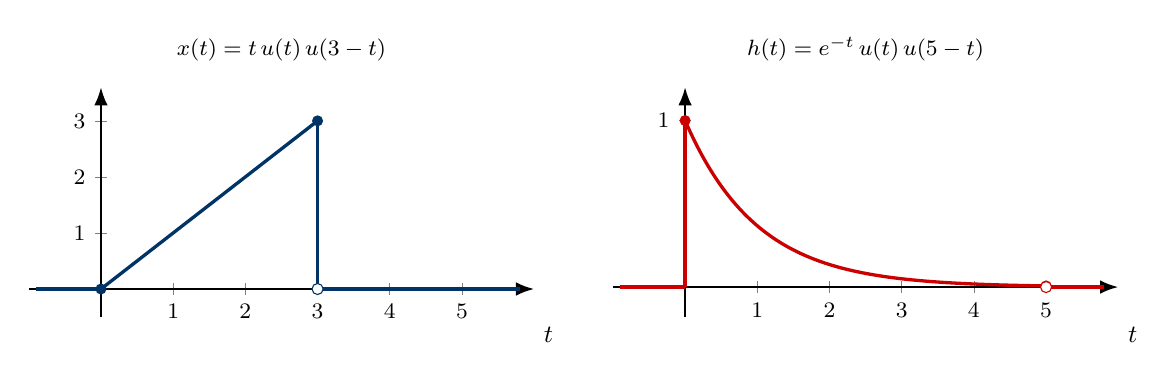
\begin{tikzpicture}[>=Latex, font=\small]

\colorlet{xcol}{utnblue}
\colorlet{hcol}{red!80!black}

% =====================================================================
% PANEL x(t)
% =====================================================================
\begin{axis}[
    name=panX,
    width=8cm, height=4.5cm,
    axis lines=center,
    xlabel={$t$},
    xlabel style={anchor=north west, at={(axis description cs:1,0)}},
    xmin=-1, xmax=6,
    ymin=-0.5, ymax=3.6,
    clip=false,
    axis line style={->, thick},
    xtick={0,1,2,3,4,5},
    ytick={0,1,2,3},
    every tick label/.style={font=\footnotesize},
    title={\footnotesize $x(t) = t\,u(t)\,u(3-t)$},
]
    % cero a la izquierda
    \addplot[xcol, very thick, domain=-0.9:0, samples=2] {0};
    % rampa en [0,3]
    \addplot[xcol, very thick, domain=0:3, samples=2] {x};
    % cero a la derecha de 3
    \addplot[xcol, very thick, domain=3:5.8, samples=2] {0};
    % salto en t=3: relleno arriba (u(0)=1 da x(3)=3), abierto abajo
    \draw[xcol, very thick] (axis cs:3,0) -- (axis cs:3,3);
    \fill[xcol]  (axis cs:3,3) circle (2pt);
    \fill[white] (axis cs:3,0) circle (2pt);
    \draw[xcol]  (axis cs:3,0) circle (2pt);
    % continuidad en t=0
    \fill[xcol] (axis cs:0,0) circle (2pt);
\end{axis}

% =====================================================================
% PANEL h(t)
% =====================================================================
\begin{axis}[
    name=panH,
    at={(panX.east)}, anchor=west, xshift=1cm,
    width=8cm, height=4.5cm,
    axis lines=center,
    xlabel={$t$},
    xlabel style={anchor=north west, at={(axis description cs:1,0)}},
    xmin=-1, xmax=6,
    ymin=-0.18, ymax=1.2,
    clip=false,
    axis line style={->, thick},
    xtick={0,1,2,3,4,5},
    ytick={0,1},
    every tick label/.style={font=\footnotesize},
    title={\footnotesize $h(t) = e^{-t}\,u(t)\,u(5-t)$},
]
    % cero a la izquierda
    \addplot[hcol, very thick, domain=-0.9:0, samples=2] {0};
    % exponencial en [0,5]
    \addplot[hcol, very thick, domain=0:5, samples=200] {exp(-x)};
    % cero a la derecha de 5
    \addplot[hcol, very thick, domain=5:5.8, samples=2] {0};
    % salto en t=0: 0->1
    \draw[hcol, very thick] (axis cs:0,0) -- (axis cs:0,1);
    \fill[hcol] (axis cs:0,1) circle (2pt);
    % salto en t=5: e^{-5}->0 (relleno arriba, abierto abajo)
    \pgfmathsetmacro{\hfive}{exp(-5)}
    \draw[hcol, very thick] (axis cs:5,0) -- (axis cs:5,\hfive);
    \fill[hcol]  (axis cs:5,\hfive) circle (2pt);
    \fill[white] (axis cs:5,0) circle (2pt);
    \draw[hcol]  (axis cs:5,0) circle (2pt);
\end{axis}

\end{tikzpicture}
\end{document}
